
\documentclass{tufte-handout}

%\geometry{showframe}% for debugging purposes -- displays the margins
\usepackage{amsmath}
%\usepackage{mparhack}
% Set up the images/graphics package
\usepackage{graphicx}
\usepackage{float}
\setkeys{Gin}{width=\linewidth,totalheight=\textheight,keepaspectratio}
\graphicspath{{graphics/}}
\title{PH5 Pre-release Materials\thanks{Freely modified from various Wikipedia pages and annotated by Joe Rowing}}
\author[]{Joe Rowing}
\date{24 April 2016}  % if the \date{} command is left out, the current date will be used

% The following package makes prettier tables.  We're all about the bling!
\usepackage{booktabs}


% The units package provides nice, non-stacked fractions and better spacing
% for units.
\usepackage{units}
\usepackage{siunitx}
% The fancyvrb package lets us customize the formatting of verbatim
% environments.  We use a slightly smaller font.
\usepackage{fancyvrb}
\fvset{fontsize=\normalsize}

% Small sections of multiple columns
\usepackage{multicol}
\newcounter{question}
% Provides  
% These commands are used to pretty-print LaTeX commands
\newcommand{\doccmd}[1]{\texttt{\textbackslash#1}}% command name -- adds backslash automatically
\newcommand{\docopt}[1]{\ensuremath{\langle}\textrm{\textit{#1}}\ensuremath{\rangle}}% optional command argument
\newcommand{\docarg}[1]{\textrm{\textit{#1}}}% (required) command argument
\newenvironment{docspec}{\begin{quote}\noindent}{\end{quote}}% command specification environment
\newcommand{\docenv}[1]{\textsf{#1}}% environment name
\newcommand{\docpkg}[1]{\texttt{#1}}% package name
\newcommand{\doccls}[1]{\texttt{#1}}% document class name
\newcommand{\docclsopt}[1]{\texttt{#1}}% document class option name


\newcommand{\parnum}{\bfseries\arabic{parcount}}

\newcounter{parcount}
\newcommand\p{%
    \stepcounter{parcount}%
    \leavevmode\marginpar[\hfill\parnum]{\parnum}%
}
\begin{document}

\maketitle% this prints the handout title, author, and date

\begin{abstract}
\noindent This document adds to the pre-release materials from WJEC and hopefully illustrates some suitable questions. 
\end{abstract}

%\printclassoptions

\section{The Big Bang Theory}

\p The Big Bang theory is the prevailing cosmological model for the early development of the universe. The key idea is that the universe is expanding. Consequently, the universe was denser and hotter in the past \sidenote{Olbers' paradox, also called the "dark night sky paradox", is worth noting here - it's the argument that the darkness of the night sky conflicts with the assumption of an infinite and eternal static universe. The darkness of the night sky is one of the pieces of evidence for a dynamic universe such as the Big Bang model. If the universe is static, homogeneous at a large scale, and populated by an infinite number of stars, any sight line from Earth must end at the (very bright) surface of a star, so the night sky should be completely bright. This contradicts the observed darkness of the night.}. Moreover, the Big Bang model suggests that at some moment
all matter in the universe was contained in a single point, which is considered the beginning of the universe. Modern measurements place this moment at approximately 13.8 billion years ago, which is thus considered the age of the universe. After the initial expansion, the universe cooled sufficiently to allow the formation of subatomic particles, including protons, neutrons, and electrons. Though simple atomic nuclei formed within the first three minutes after the Big Bang, thousands of years passed before the first electrically neutral atoms formed. The majority of atoms produced by the Big Bang were hydrogen, along with helium and traces of lithium (see figure 1) \begin{marginfigure} 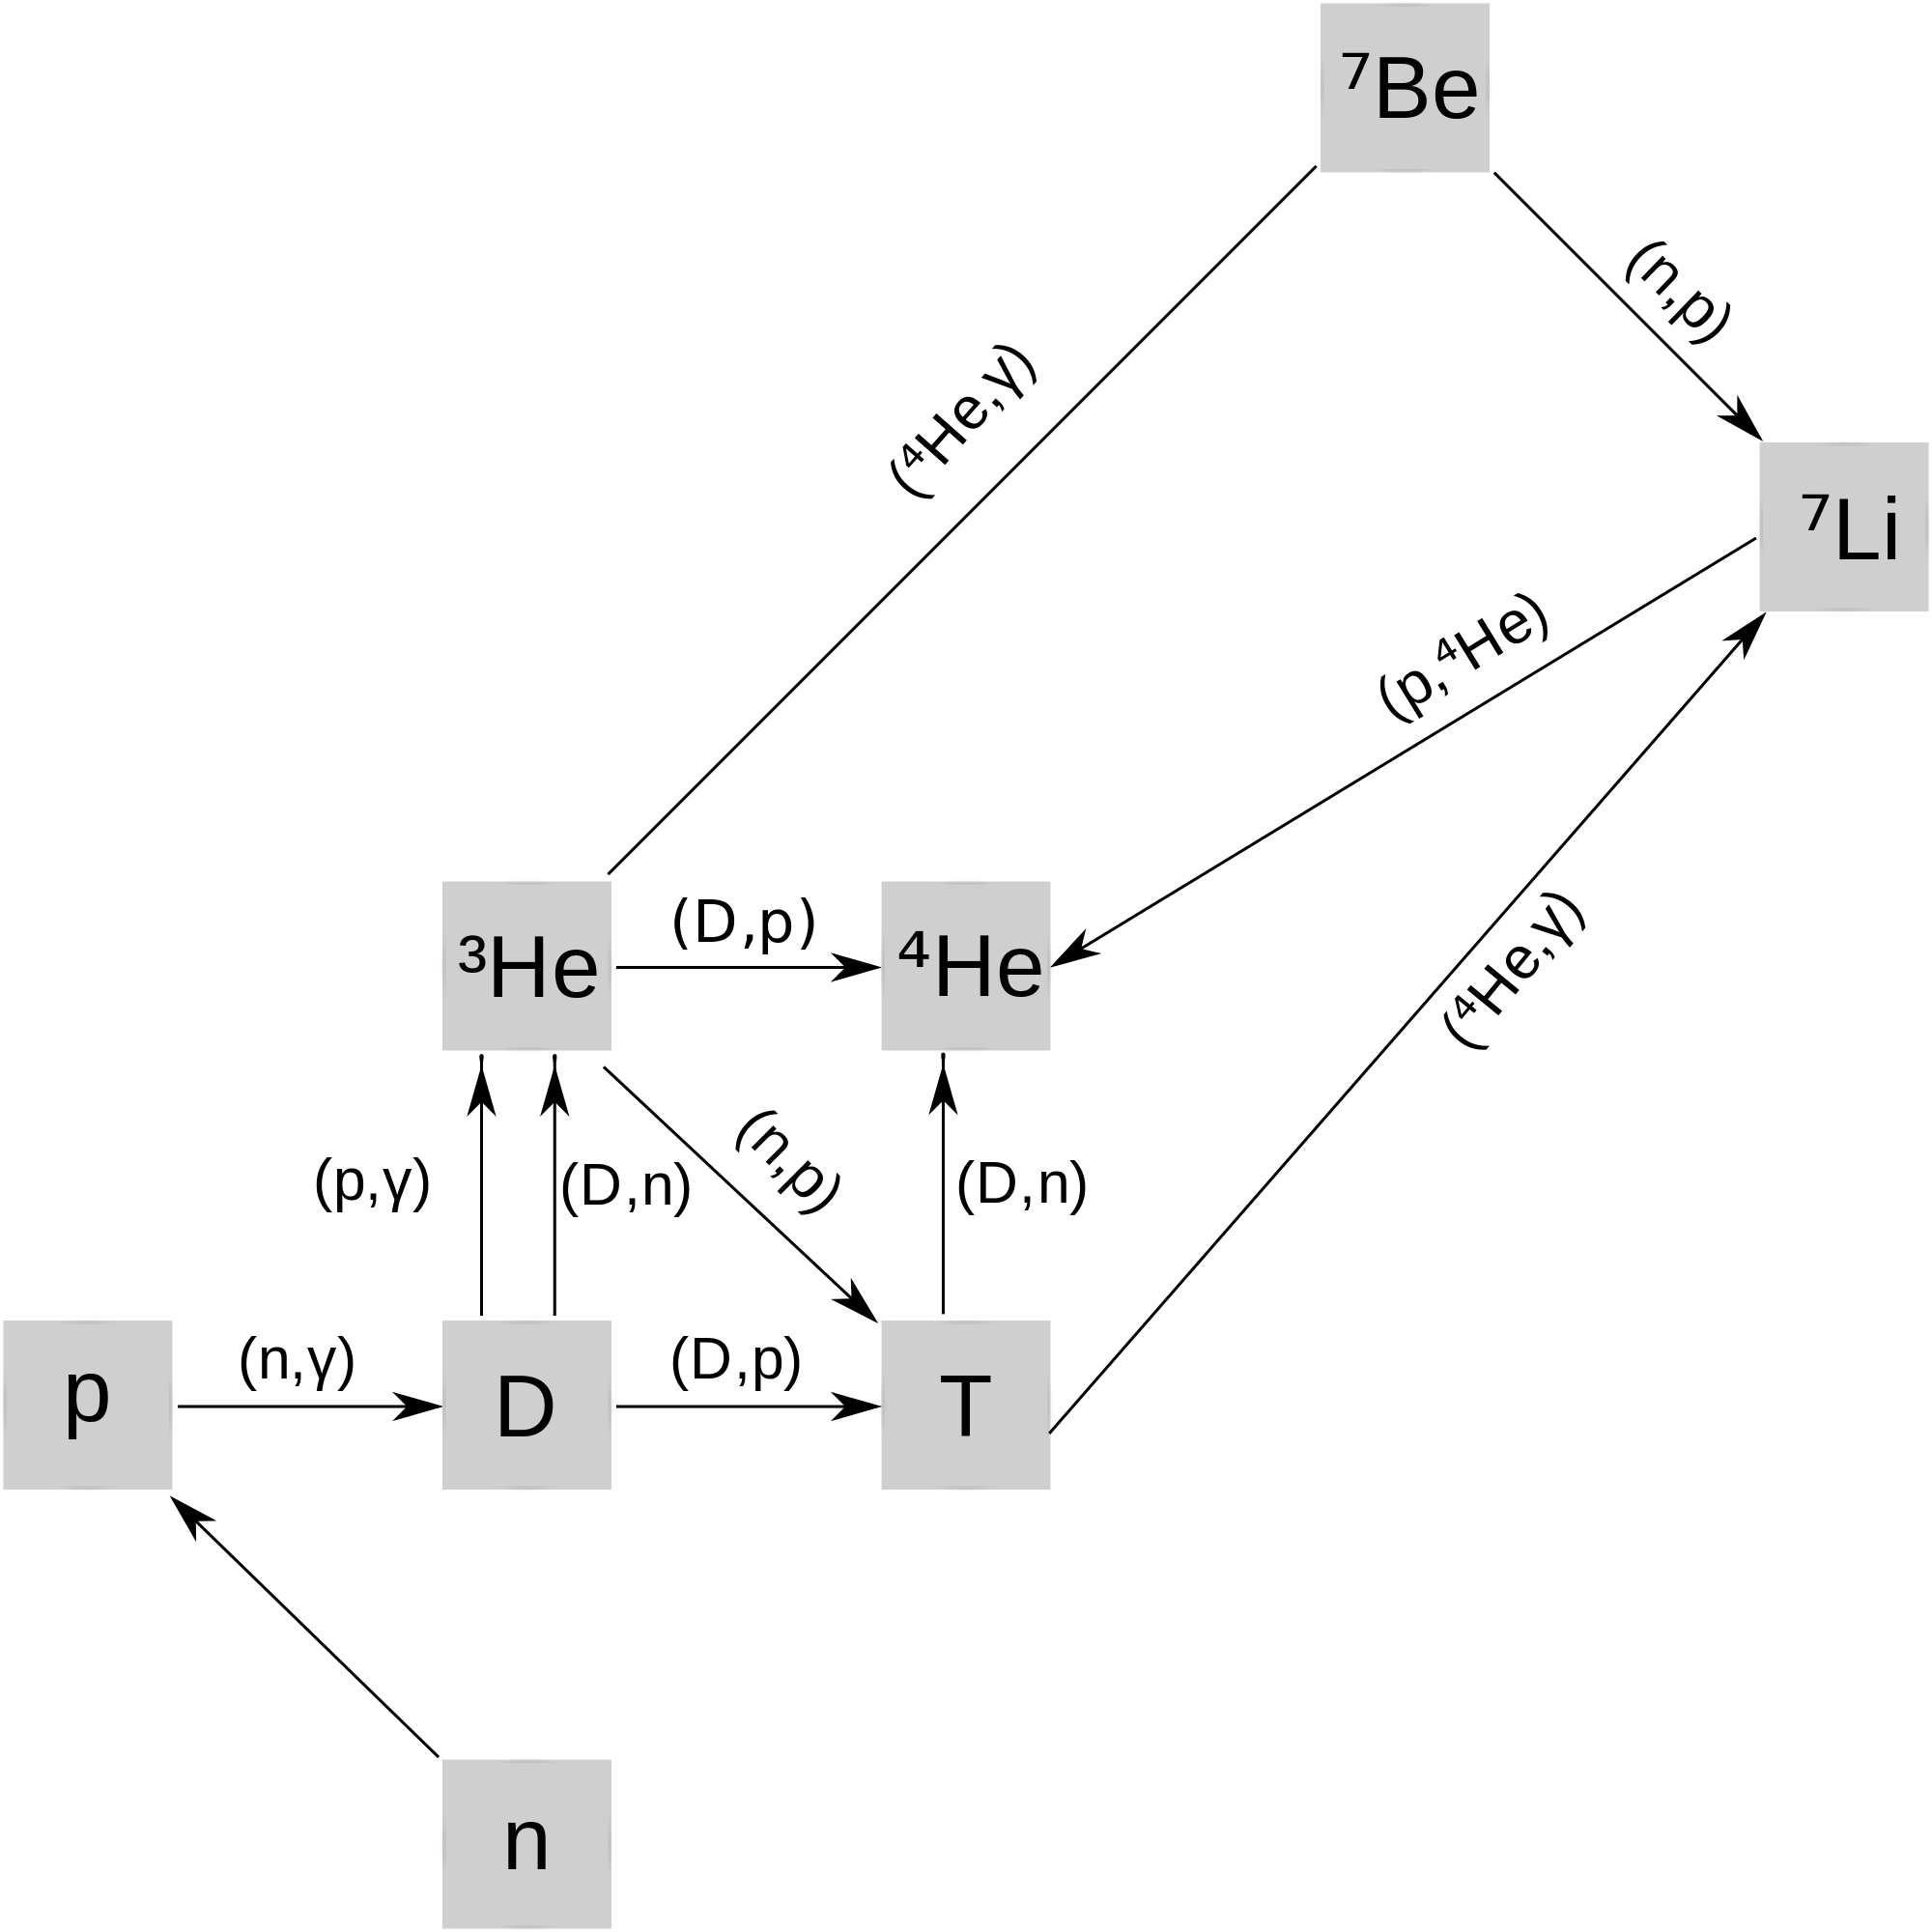
\includegraphics{nucleo_svg.png} \caption{Big Bang Nucleosynthesis took place via twelve nuclear interactions that produced three isotopes of hydrogen, two of helium, and one isotope each of lithium and beryllium. Presumably the Be-7 that was produced is not mentioned here because it has a halflife of only 53d. Free neutrons were also produced, but their half-life is even shorter, at only 10.6min} \end{marginfigure}. Giant clouds of these primordial elements later coalesced through gravity to form stars and galaxies, and the heavier elements were synthesized either within stars or during supernovae.
 
 
\p The Big Bang theory offers a comprehensive explanation for a broad range of observed phenomena, including the abundance of light elements, the cosmic microwave background radiation (CMBR), large scale structure, and Hubble's Law. Today, the distances between galaxies is increasing hence, in the past, galaxies were closer together. The known laws of nature can be used to calculate the characteristics of the universe in detail back to a
time when densities and temperatures were extreme. While large particle accelerators can replicate such conditions, resulting in confirmation and refinement of the details of the Big Bang model, these accelerators can only probe so far into high energy conditions. 
Consequently, the state of the universe in the earliest instants of the Big Bang expansion is poorly understood and still an area of open investigation. The Big Bang theory does not provide any explanation for the initial conditions of the universe; rather, it describes and explains the general evolution of the universe going forward from that point on\sidenote{It is tempting to ask what came``before the Big Bang'', but the Big Bang was both the creation of space and time, so this is a bit like asking what colour physics is.}.
\p Belgian Catholic priest and scientist Georges Lemaitre proposed what became the Big Bang theory \sidenote{English astronomer Fred Hoyle is credited with coining the term "Big Bang" during a 1949 BBC radio broadcast. It is popularly reported that Hoyle, who favoured an alternative "steady state" cosmological model, intended this to be pejorative, but Hoyle explicitly denied this and said it was just a striking image meant to highlight the difference between the two models} in 1927. Over time, scientists built on his initial idea of cosmic expansion, which, his theory went, could be traced back to the origin of the cosmos and which led to the formation
of the modern universe. The framework for the Big Bang model relies on Albert Einstein's theory of general relativity and on simplifying assumptions such as homogeneity and isotropy
of space. In 1929, Edwin Hubble discovered that the distances to faraway galaxies were strongly correlated with their red shifts. Hubble's observation was taken to indicate that all distant galaxies and clusters have an apparent velocity directly away from our vantage point: that is, the farther away, the higher the apparent velocity, regardless of direction. The interpretation is that all observable regions of the universe are receding from each other.
\p While the scientific community was once divided between supporters of two different expanding universe theories - the Big Bang and the Steady State theory - observational confirmation of the Big Bang scenario came with the discovery of the CMBR in 1964, and
later when its spectrum was found to match that of thermal radiation from a black body.
\section{The History of the Universe}
\subsection{Inflation}
\p The earliest phases of the Big Bang are subject to much speculation. In the most common models the universe was filled homogeneously\sidenote{Uniform in structure or composition throughout, as of a chemical mixture.} and isotropically\sidenote{To exhibit the same properties or behaviour in all directions} with an incredibly high energy density and huge temperatures and pressures and was very rapidly expanding and cooling. Approximately $10^{-37}$ seconds into the expansion, a phase transition caused a cosmic inflation, during which the universe grew exponentially. After inflation stopped, the universe consisted of a quark-gluon plasma, as well as all other elementary particles. Temperatures were so high that the random motions of particles were at relativistic speeds, and particle-antiparticle
pairs of all kinds were being continuously created and destroyed in collisions. At some point baryogenesis, a reaction that we know little about, violated the conservation of baryon number, leading to a very small excess of quarks and leptons over antiquarks and antileptons - of the order of one part in 30 million. This resulted in the predominance of matter over antimatter in the present universe.
\begin{figure}
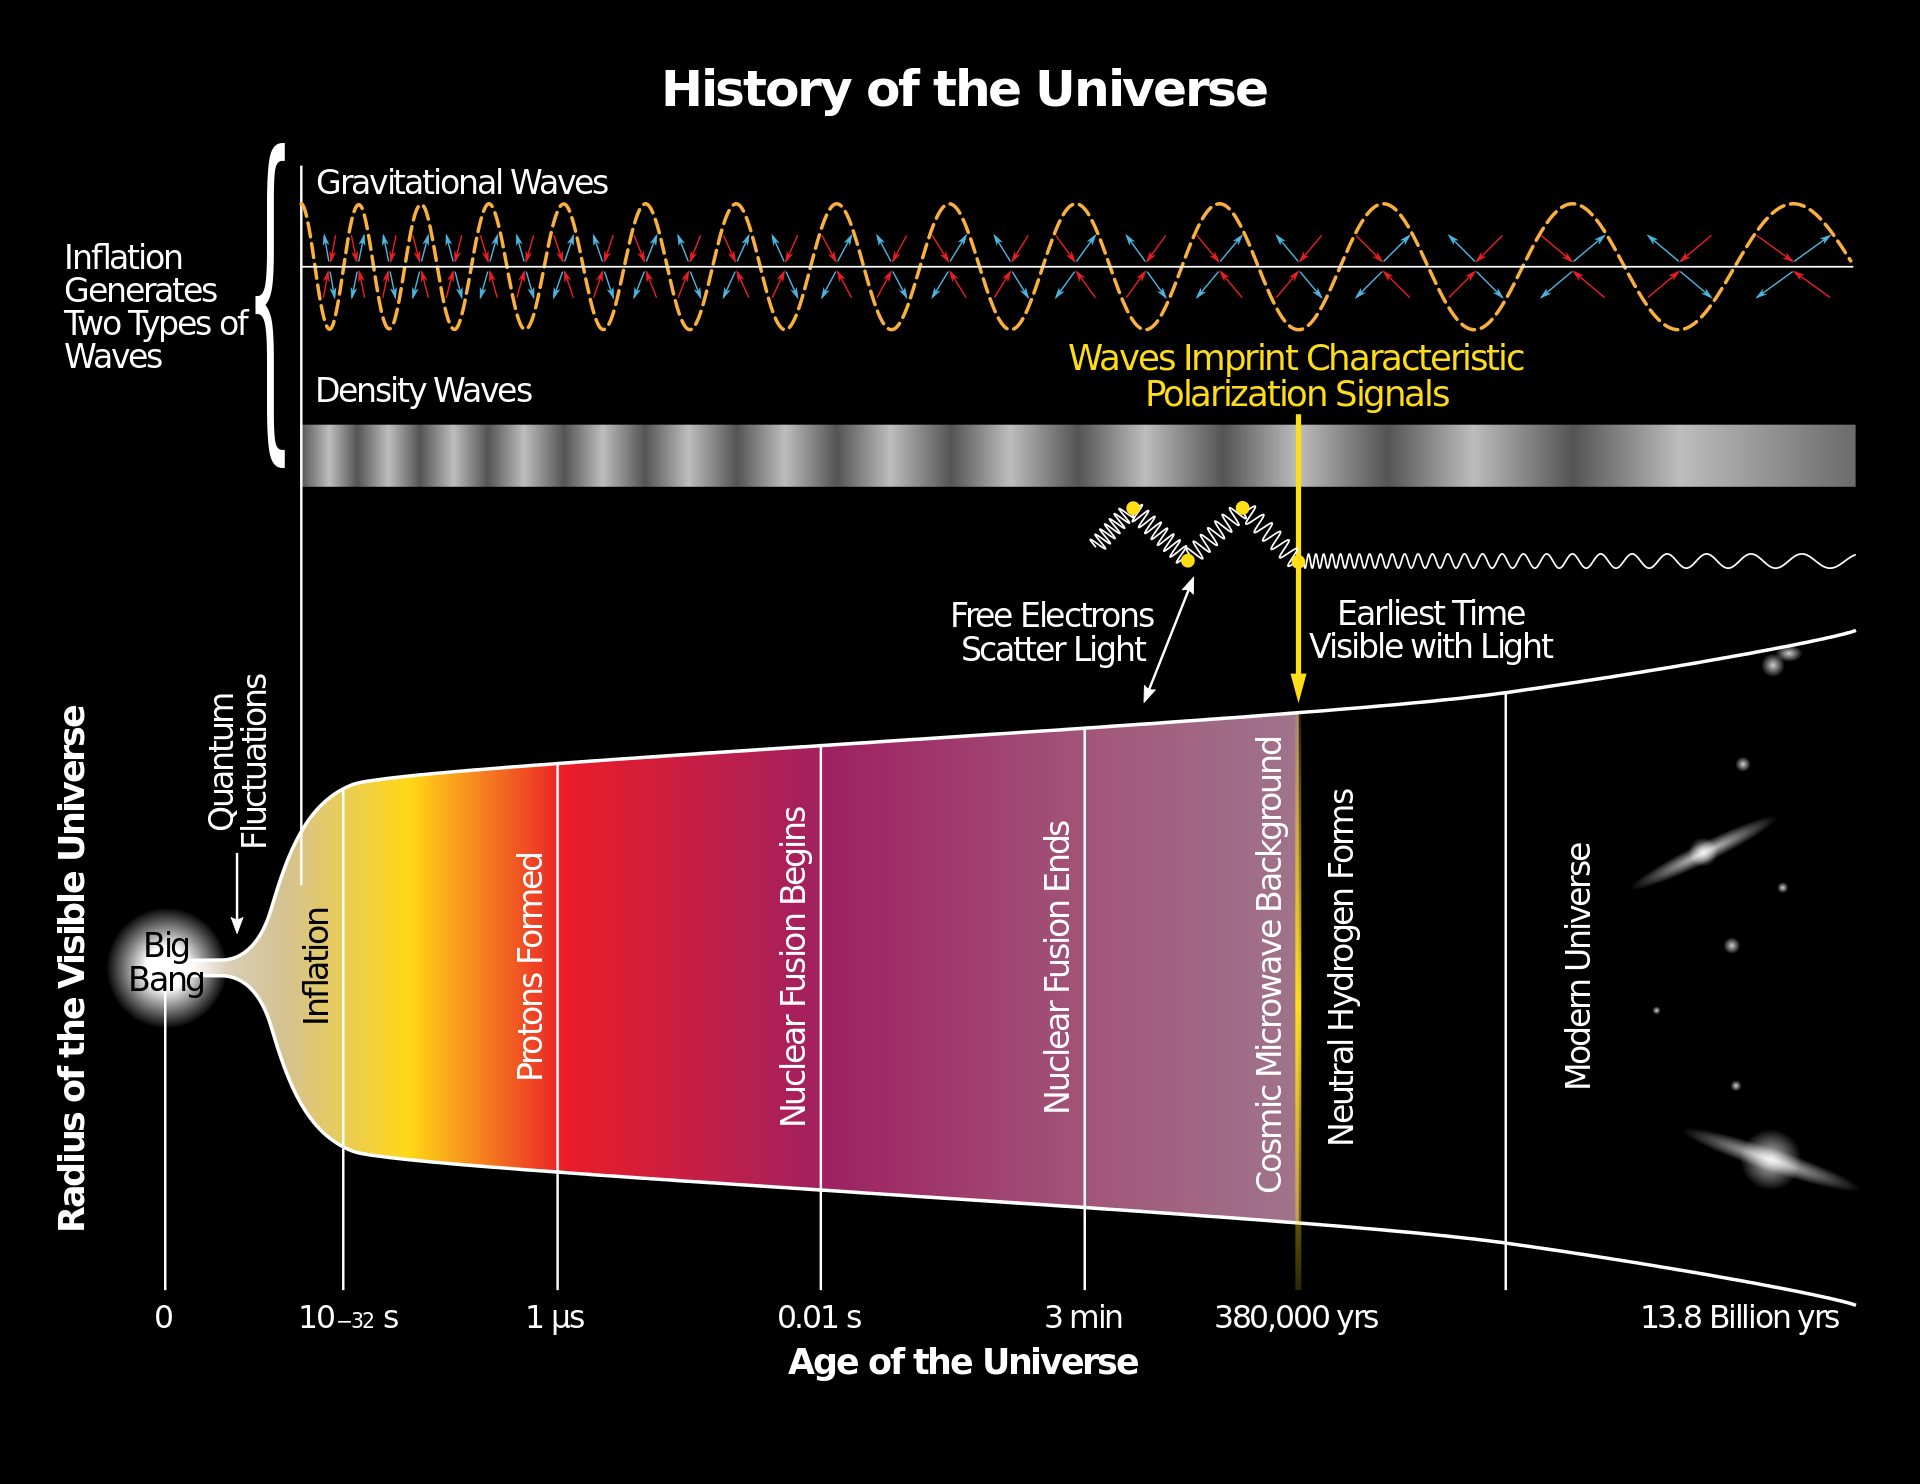
\includegraphics[]{History_of_the_Universe_svg.png}
\caption{History of the Universe}
\end{figure} 


\subsection{Protons Forming}
\p The universe continued to decrease in density and fall in temperature, hence the typical energy of each particle was decreasing. After about $10^{-11}$ seconds, the picture becomes less speculative, since particle energies drop to values that can be attained in particle physics experiments. At about $10^{-6}$ seconds, quarks and gluons combined to form baryons such as protons and neutrons. The small excess of quarks over antiquarks led to a small excess of baryons over antibaryons. The temperature was now no longer high enough to create new proton-antiproton pairs (similarly for neutrons-antineutrons), so a mass annihilation
immediately followed, leaving just one in $10^{10}$ of the original protons and neutrons, and none of their antiparticles. A similar process happened at about 1 second for electrons and positrons. After these annihilations, the remaining protons, neutrons and electrons were no longer moving relativistically and the energy density of the universe was dominated by photons (with a minor contribution from neutrinos).

\subsection{Nuclear Fusion Begins and Ends}
\p A fraction of a second into the expansion, when the temperature was about a hundred billion kelvin (100 GK), neutrons combined with protons to form the universe's deuterium and helium nuclei in a process called Big Bang nucleosynthesis. However, around 3 minutes after the Big Bang the universe had cooled further so that fusion was no longer possible. The Big Bang theory itself predicts mass abundances of about 75\% of hydrogen-1, about 25\% helium-4, about 0.01\% of deuterium,\sidenote{Question Expect a question on binding energy} trace amounts (in the order of \num{e-10}) of lithium and beryllium, and no other heavy elements\sidenote{Question Descrive how the heavier elements are formed}. That the observed abundances in the universe are generally consistent with these abundance numbers is considered strong evidence for the Big Bang theory.
\subsection{The Universe Becomes Transparent}
\p After about 380 000 years the universe cooled to a temperature of around 3 000 K. The electrons and nuclei combined into atoms (mostly hydrogen). This meant that radiation could travel freely without forcing free charges to oscillate and continued through space largely unimpeded. This relic radiation is known as the CMBR. It is frequently stated that the CMBR that is detected today started as gamma radiation shortly after the Big Bang. This is not strictly true because these photons were scattered and absorbed a long time ago. The CMBR that we can detect now started as mainly infra-red radiation 380 000 years after the Big Bang when the universe suddenly became transparent. Although the universe previously had been hot enough to emit gamma rays (as a black body radiator), this radiation was not able to travel very far.

\subsection{The Modern Universe and The Big Bang Theory}
\p In today's universe, the earliest and most direct observational evidence of the validity of the theory are the expansion of the universe according to Hubble's law (as indicated by the red shifts of galaxies), discovery and measurement of the CMBR and the relative abundances of light elements produced by Big Bang nucleosynthesis. More recent evidence includes
observations of galaxy formation and evolution, and the distribution of large-scale cosmic structures. These are sometimes called the ``four pillars'' of the Big Bang theory. 
\p Observations of distant galaxies and quasars show that these objects are red shifted - the light emitted from them has been shifted to longer wavelengths.\begin{marginfigure} 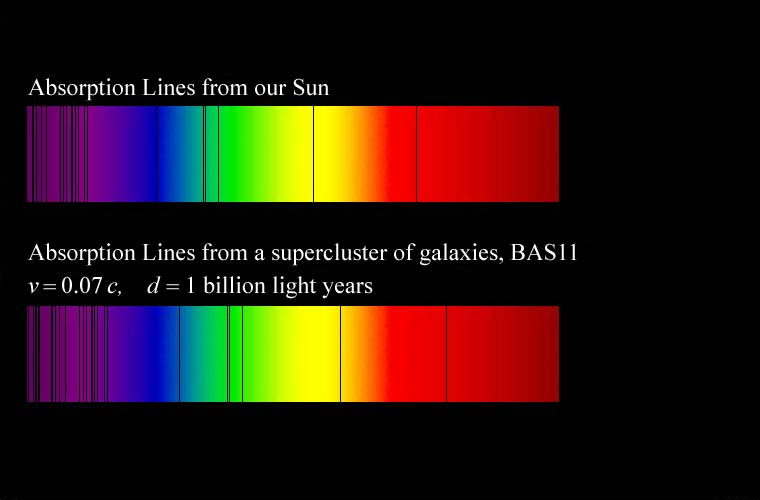
\includegraphics{redshift.jpg} \caption{redshift} \end{marginfigure}\sidenote{Doppler's formula, $\frac{\Delta \lambda}{\lambda_{0}}=\frac{v}{c}$, links the frequency shift with the velocity of the source} This can be seen by taking a frequency spectrum of an object and matching the spectroscopic pattern of emission lines or absorption lines corresponding to atoms of the chemical elements interacting with the light.
These red shifts are distributed evenly among the observed objects in all directions. If the red shift is interpreted as a Doppler shift, the recessional velocity of the object can be calculated.
When the recessional velocities are plotted against these distances, a linear relationship known as Hubble's law is observed:
\begin{equation*}\tag{Equation 1}
v=H_{0}D
\end{equation*}
where:
\begin{itemize}
\item $v$ is the recessional velocity of the galaxy or other distant object;
\item $D$ is the distance to the object;
\item $H_0$ is the Hubble constant \sidenote{$H_0$, the Hubble constant, is one of the least well-known of the physical constants; at various points it has been estimated to be anywhere between $50-90 kms^{-1} pc{-1}$. The value with the lowest error is currently that of the Planck Collaboration (see http://arxiv.org/abs/1303.5062): $(67.2 \pm 1.2)kms^{-1}pc^{-1}$}, measured to be \SI{2.2685e-18}{\per\second}.
\end{itemize}
If Hubble's law, $v = H_{0}D$, is combined with a simple calculation for the escape velocity from a spherical universe, the so-called critical density of the universe can be calculated:

\begin{equation*}\tag{Equation 2}
\frac{1}{2}mv^{2}_{esc} - \frac{GMm}{R}=0
\end{equation*}
\p where $v_{esc}$ is the escape velocity of an arbitrary mass, $m$, which is a distance, $R$, from the 'centre' of the universe and $M$ is the mass of the universe contained inside the sphere of radius $R$ (upon whose surface the arbitrary mass lies). When the volume of the sphere of
radius $R$ is also included, this leads to:
\begin{equation*}\tag{Equation 3}
\rho_{c} =\frac{3H^{2}_{0}}{8 \pi G} 
\end{equation*}
\p The critical density, $\rho_{c}$ , \sidenote{If the density of matter in the Universe is high (a closed Universe), self-gravity slows the expansion until it halts, and ultimately re-collapses.
If the density of matter in the Universe is low (an open Universe), self-gravity is insufficient to stop the expansion, and the Universe continues to expand forever (albeit at an ever decreasing rate).
Balanced on a knife edge between Universes with high and low densities of matter, there exists a critical density Universe, where the expansion is halted only after an infinite time.
The density parameter is usually used to make comparisons between these models and is defined as:
\[ \Omega \equiv \frac{\rho}{\rho_{c}} = \frac{8 \pi G \rho }{3 H^{2}} \] } of the universe can be calculated from this equation and corresponds to 5 hydrogen atoms per cubic metre.
\p Not only can we calculate a mean density for the modern universe, we can also calculate a mean temperature. From the CMBR, if the universe is assumed to be a black body then a temperature of ${2.725 \pm 0.001}$K is obtained. Moreover, the microwave spectrum follows a perfect black body spectrum shape. See Figure \ref{cobe}
\newpage
\begin{figure}
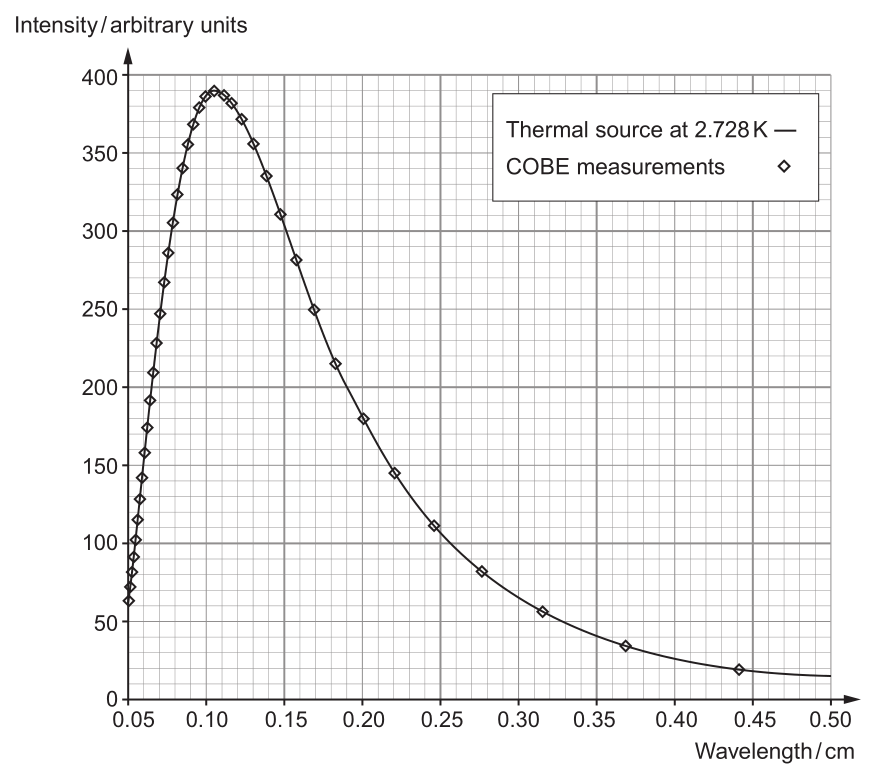
\includegraphics{cobedata.png}
\caption{Comparison between the predicted spectrum of the cmbr (line) and the spectrum as measured by cobe (diamonds).} \label{cobe}
\end{figure}

\p Since the early 1980s more and more evidence for larger scale order of matter in the universe has been discovered. Stars are organised into galaxies, which in turn form galaxy groups, galaxy clusters, super-clusters, sheets, walls and filaments, which are separated by immense voids, creating a vast foam-like structure sometimes called the ``cosmic web''. All these enormous scale structures have been simulated by computer and all seem to agree with the Big Bang theory\ldots

\begin{figure}
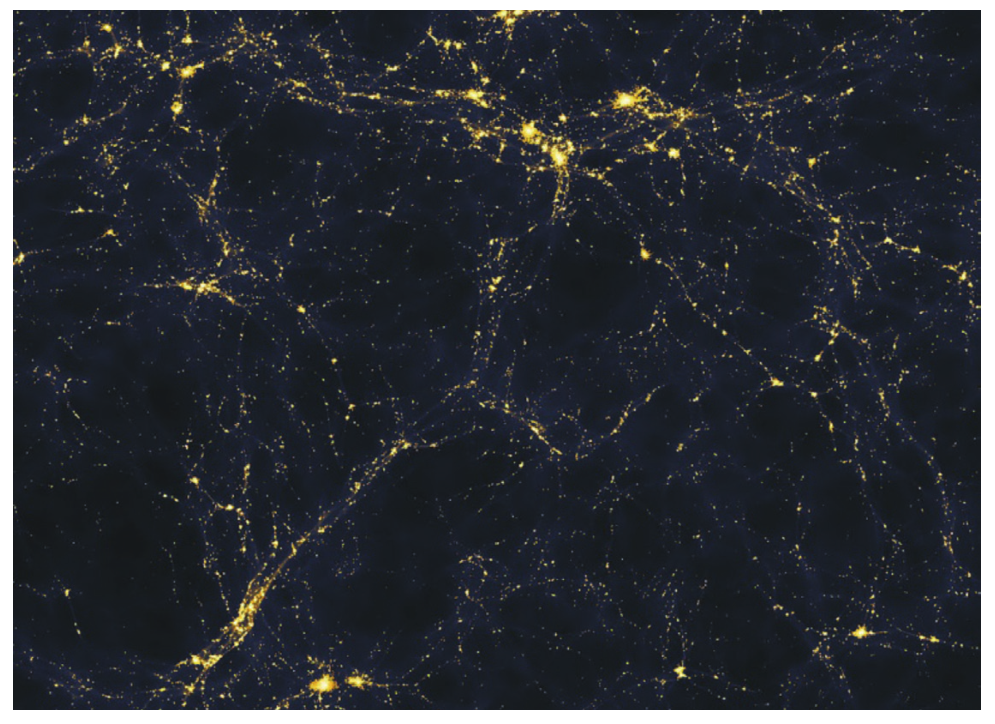
\includegraphics{cosmicweb.PNG}
\caption{Cosmic Web}
\end{figure} 
\begin{fullwidth}
\newpage
\section{Practice Questions:}
Where necessary, use the values for constants provided in the wjec formula booklet
\begin{enumerate}
\item Explain the following terms in your own words: 
\begin{enumerate}
\item cosmic microwave background radiation 
\item redshift \item homogeneity (as it applies in this context) \item black body \item inflation \item annihilation \item relativistic speeds \item baryogenesis \item quark \item lepton \item gluon \item quasar \item Hubble constant \item Doppler shift \item recessional velocity \item escape velocity 
\item critical density 
\item galactic supercluster 
\end{enumerate}
\item What limits our ability to simulate conditions in the earliest moments of the Big Bang? 
\item What is the minimum energy is required to cause a proton-antiproton pair creation event?
\item In Big Bang nucleosynthesis there are two processes by which neutrons interact to create protons: \[n+e^{+} \leftrightarrow v_{e} + p\] \[n + \bar{v_{e}} \leftrightarrow p+e^{-}\] 
Show that both of these processes conserve charge, baryon number and lepton number. 
\item The cmbr has a black body temperature of $(2.725 \pm 0.001)K.$
\begin{enumerate}
\item What is the peak frequency of the radiation emitted by the cosmic microwave background? 
\item What is the uncertainty in this frequency? 
\item What would the peak wavelength be at 380000yr after the Big Bang, and in which part of the electromagnetic spectrum would this lie? 
\end{enumerate}

\item Describe the structure of baryons, and give three examples. 
\item Why did the Universe become transparent? 
\item A bright sodium line at 589.995nm is observed from the smaller star of a binary system to be oscillating between 678.789nm and 678.200nm. 
\begin{enumerate}
\item At what speed is the binary system moving away from Earth?
\item At what speed is the smaller star orbiting the larger star?
\end{enumerate}
\item Edwin Hubble's first value for the Hubble constant was $500kms^{-1}Mpc^{-1}$.
\begin{enumerate}
\item Show that the standard unit for the Hubble constant ($kms^{-1} Mpc^{-1}$) has the same units as the unit quoted in the text $(s^{-1})$. 
\item Convert Hubble's first value of the Hubble constant to $s^{-1}$. 
\end{enumerate}
\item Using the value of $H_{0}$ provided, calculate the recessional velocity (as a fraction of the speed of light) of the quasar 3C 273 which lies 2.443 gigalightyears from Earth. 
\item Using your existing knowledge of gravitational fields: 
\begin{enumerate}
\item Derive Equation 2. 
\item Derive Equation 3.
\end{enumerate}
\item Calculate the critical density of the Universe in $kgm^{-3}$ and show that this is approximately ``5 hydrogen atoms per cubic metre''.

\end{enumerate}


\end{fullwidth}
\end{document}
\section{Answers}
Answers
1. No answers provided 2. Our ability to simulate the conditions in the earliest moments of the Big Bang is limited by the energies achievable in particle accelerators.
3. (a)
n e+ νe p Q 0 +1 0 +1 B +1 0 0 +1 L 0 −1 −1 0
(b)
n νe p e− Q 0 0 +1 −1 B +1 0 +1 0 L 0 +1 0 +1 4. (a) Using Wein‘s Law:
λpeak =
b T
c f
=
2.90×10−3 mK 2.725K
3.00×108 ms−1 f
= 1.06×10−3 m
f =
3.00×108 ms−1 1.06E−3 f = 282×109 s−1 f = 282GHz
(b) The percentage error in the peak frequency will be the same as the percentage error in the temperature of the cosmic microwave background (we assume that there is no error in the values of the constants provided).
σT =
uncertainty actual value
σT =
0.001K 2.725K σT = 3.67×10−4 = 0.0367% σf = 0.0367% σf = 0.0367%×282GHz σf = ±103MHz Therefore f = (281.897±0.103)GHz.
DRAFT FOR REVIEW
the big bang theory 10
(c) Again using Wein‘s Law, and the value of 3000K from the text
λpeak =
b T
λpeak =
2.90×10−3 mK 3000K λpeak = 9.67×10−7 m λpeak = 967nm Given that the visible spectrum runs from approximately 390–700nm this would be in the infrared part of the spectrum. 5. Baryons are particles composed of three quarks. Examples of baryons include protons, neutrons, the delta baryons (∆++, ∆+, ∆0 and ∆−), the lambda baryons (Λ0, Λ0 b, Λ+ c and Λ+), etc. 6. The Universe became transparent because electrons, which had previously scattered photons (via Thompson scattering), became bound to protons to form neutral hydrogen. 7. (a) To calculate the recessional velocity of the binary system we find the mid-point (i.e. the average) of the two wavelengths – this is the wavelength that would be measured if the stars were not orbiting each other.
λrecession =
678.789nm+678.200nm 2 λrecession = 678.495nm Using this wavelength in the equation for Doppler shift yields the recessional velocity: ∆λ λ = v c 678.495nm−589.995nm 589.995nm = v 3.00×108 ms−1 0.150001 = v 3.00×108 ms−1 v = 0.150001×3.00×108 ms−1 v = 45.0×106 ms−1 (a) To calculate the orbital velocity, we use the difference between either of the received wavelengths and lab wavelength. ∆λ λ = v c 678.789nm−589.995nm 678.495nm = v 3.00×108 ms−188.7940nm 589.995nm = v 3.00×108 ms−1 0.150500 = v 3.00×108 ms−1 v = 0.150500×3.00×108 ms−1 v = 45.150×106 ms−1
DRAFT FOR REVIEW
the big bang theory 11
When we remove the recessional component from this we are left with the orbital velocity: vorbital = 0.150×106 ms−1 or 150kms−1. 8. (a) The kilometre and parsec are both units of distance. kms−1 Mpc−1 = s−1 ms−1 m−1 = s−1 s−1 = s−1 (b) One parsec is 3.09×1016 m. H0 = 500kms−1 1Mpc
H0 =
500×103 ms−1 3.09×1016 m H0 = 1.62×10−11 s−1 9. 2.443×109 lightyears is 2.443×109×3.00×108 ms−1×365×24×60×60 = 2.31×1025 m. v = H0D v = 2.2685×10−18 s−1×2.31×1025 m v = 52.4Mms−1 v = 0.174c
10. (a) The gravitational potential (VG) of an object with mass m at radius R from a body with mass M is: VG = −GM/R. The gravitational potential energy of this object is then U = GMm/R. In order to escape the gravitational field of mass M, the object must have kinetic energy equal to U, which yields Equation 2. 1 2 mv2esc = GMm R 1 2 mv2esc− GMm R = 0
(b) The density of the Universe is ρ = M/V. Beginning with Equation 2: GMm R = 1 2 mv2 M = Rv2 2G We now substitute in our equation for v in terms of Hubble‘s constant and the radius of the Universe v = H0R, and divide by the volume of the Universe V = 4/3πR3.
M =
RH2 0R2 2G
M V
=
H2 0R3/2G 4/3πR3
ρ =
3H2 0 8πG
DRAFT FOR REVIEW
the big bang theory 12
11. Using the equation provided:
ρc =
3H2 0 8πG
ρc =
3×2.2685×10−18 s−128 π×6.67×10−11 Nm2 kg−2
ρc =
3×5.15×10−36 s−2 1.68×10−9 Nm2 kg−2
ρc =
3×1.54×10−35 s−2 1.68×10−9 kg−1 m3 s−2 ρc = 9.21×10−27 kgm−3 The mass of a hydrogen atom is equal to the mass of a proton plus the mass of an electron:
mH = mp +me mH = 1.66×10−27 kg+9.11×10−31 kg mH = 1.66×10−27 kg Therefore, in terms of hydrogen masses, the critical density is:
ρc =
9.21×10−27 kgm−3 1.66×10−27 kg ρc = 5.55kg−1